\documentclass[a4paper,11pt]{article}
\usepackage[utf8]{inputenc}
\usepackage[spanish]{babel}
\usepackage[affil-it]{authblk}
\usepackage{enumerate}
\usepackage{graphicx}
\usepackage{listings}
\usepackage{hyperref}
\usepackage{amsmath}
\usepackage{amssymb}
\usepackage{cancel}
\usepackage[usenames, dvipsnames]{color}
\usepackage{tikz}
\usepackage[labelfont=bf]{caption}
\usepackage{subcaption} %Multiple images
\usepackage{multicol} % Multiple columns
\usepackage{float}
\usepackage{cleveref}
\usepackage{relsize} % bigger math symbols
\usepackage[margin=1.1in]{geometry}
\usepackage[titletoc,toc,title]{appendix}
\usepackage{enumitem}
\usepackage{etoolbox}
\usepackage{mdframed} %frame theorems
\usetikzlibrary{calc}
\numberwithin{equation}{section}

% Footnotes with symbols

\makeatletter
\def\@fnsymbol#1{\ensuremath{\ifcase#1\or \dagger\or \ddagger\or
   \mathsection\or \mathparagraph\or \|\or **\or \dagger\dagger
   \or \ddagger\ddagger \else\@ctrerr\fi}}
\makeatother

\renewcommand{\thefootnote}{\fnsymbol{footnote}}

%Styling for code
\definecolor{codegreen}{rgb}{0,0.6,0}
\definecolor{codegray}{rgb}{0.5,0.5,0.5}
\definecolor{codepurple}{rgb}{0.58,0,0.82}
\definecolor{backcolour}{rgb}{0.95,0.95,0.92}
 
\lstdefinestyle{mystyle}{
    backgroundcolor=\color{backcolour},   
    commentstyle=\color{codegreen},
    keywordstyle=\color{magenta},
    numberstyle=\tiny\color{codegray},
    stringstyle=\color{codepurple},
    basicstyle=\footnotesize,
    breakatwhitespace=false,         
    breaklines=true,                 
    captionpos=b,                    
    keepspaces=true,                 
    numbers=left,                    
    numbersep=5pt,                  
    showspaces=false,                
    showstringspaces=false,
    showtabs=false,                  
    tabsize=2
}
 
\lstset{style=mystyle}

% Cool letters 
%Filename:      Typocaps.fd
%Created by:    MLO
%Creation date: 2003/04/02

% This file should be put in a TeX input directory

\ProvidesFile{Typocaps.fd}
   [2003/04/02 Font definition file for U/Typocaps]

\DeclareFontFamily{U}{Typocaps}{}

\DeclareFontShape{U}{Typocaps}{xl}{n}{
   <-> Typocaps
}{}

\endinput


% Footer
\usepackage{fancyhdr}
\pagestyle{fancy}
\fancyhf{}
\cfoot{\fontsize{15pt}{15pt}\usefont{U}{Typocaps}{xl}{n} 
gigantium humeris insidentes}

% Big Pictures
\usepackage[export]{adjustbox}

% Enviroment for theorems
\newmdtheoremenv[frametitle=Teorema]{theo}{Theorem}

% Circled words
\newcommand{\circled}[2][]{%
  \tikz[baseline=(char.base)]{%
    \node[shape = circle, draw, inner sep = 1pt]
    (char) {\phantom{\ifblank{#1}{#2}{#1}}};%
    \node at (char.center) {\makebox[0pt][c]{#2}};}}
\robustify{\circled}

%Appendices in spanish
\renewcommand{\appendixname}{Ap\'endices}
\renewcommand{\appendixtocname}{Ap\'endices}
\renewcommand{\appendixpagename}{Ap\'endices}

%Zero delimiter
\newcommand{\zerodel}{.\kern-\nulldelimiterspace}

%Columns separation
\setlength{\columnsep}{1cm}

%Indentation
\setlength{\parindent}{0ex}

%Multiple References

\crefrangelabelformat{equation}{(#3#1#4--#5\crefstripprefix{#1}{#2}#6)}

\usepackage{xparse}

%Boxes

\newcommand*{\boxcolor}{blue}
\makeatletter
\renewcommand{\boxed}[1]{\textcolor{\boxcolor}{%
\tikz[baseline={([yshift=-1ex]current bounding box.center)}] \node [rectangle, minimum width=1ex,rounded corners,draw] {\normalcolor\m@th$\displaystyle#1$};}}
 \makeatother

%Constantes
\newcommand{\euler}{\mathrm{e}}
\newcommand{\im}{i}

%Lemas, teoremas, definiciones y pruebas
\newcommand{\definicion}{\textbf{Definición: }}
\newcommand{\lema}{\textbf{Lema: }}
\newcommand{\teorema}{\textbf{Teorema: }}
\newcommand{\prueba}{\textbf{Prueba: }}
\newcommand{\proposicion}{\textbf{Proposición: }}
\newcommand{\corolario}{\textbf{Corolario: }}

% Definición de las secciones y su numeración

\makeatletter
\def\@seccntformat#1{%
  \expandafter\ifx\csname c@#1\endcsname\c@section\else
  \csname the#1\endcsname\quad
  \fi}
\makeatother

\begin{document}

\begin{titlepage}
\thispagestyle{fancy}

\newcommand{\HRule}{\rule{\linewidth}{0.5mm}} % Defines a new command for the horizontal lines, change thickness here

\center % Center everything on the page
 
%----------------------------------------------------------------------------------------
%	HEADING SECTIONS
%----------------------------------------------------------------------------------------

\textsc{\LARGE Universidad Nacional Autónoma de México}\\[0.3cm] % Name of your university/college

%----------------------------------------------------------------------------------------
%	LOGO SECTION
%----------------------------------------------------------------------------------------


\includegraphics[scale=0.17]{unam}

%----------------------------------------------------------------------------------------
%	SUBHEADING SECTIONS
%----------------------------------------------------------------------------------------

\textsc{\Large Electrodinámica Clásica}\\[0.3cm] % Major heading such as course name
\textsc{\large Semestre 2016-II}\\[0.3cm] % Minor heading such as course title
\textsc{\large 7 de abril de 2016}\\ % Minor heading such as course title

%----------------------------------------------------------------------------------------
%	TITLE SECTION
%----------------------------------------------------------------------------------------

\HRule \\[0.1cm]
{ \huge \bfseries Tarea \# 6. \\ Ondas electromagnéticas planas \\
y propagación de ondas.}\\ % Title of your document
\HRule \\[0.1cm]
 
%----------------------------------------------------------------------------------------
%	AUTHOR SECTION
%----------------------------------------------------------------------------------------
\setcounter{footnote}{0}
\center
\large
\emph{Autor:} \\ % Your name
\Large Favio \textsc{Vázquez}\footnote[1]{\href{mailto:favio.vazquez@correo.nucleares.unam.mx}{favio.vazquez@correo.nucleares.unam.mx}}
\\[0.7cm]
%----------------------------------------------------------------------------------------
%	COOL IMAGE SECTION
%----------------------------------------------------------------------------------------

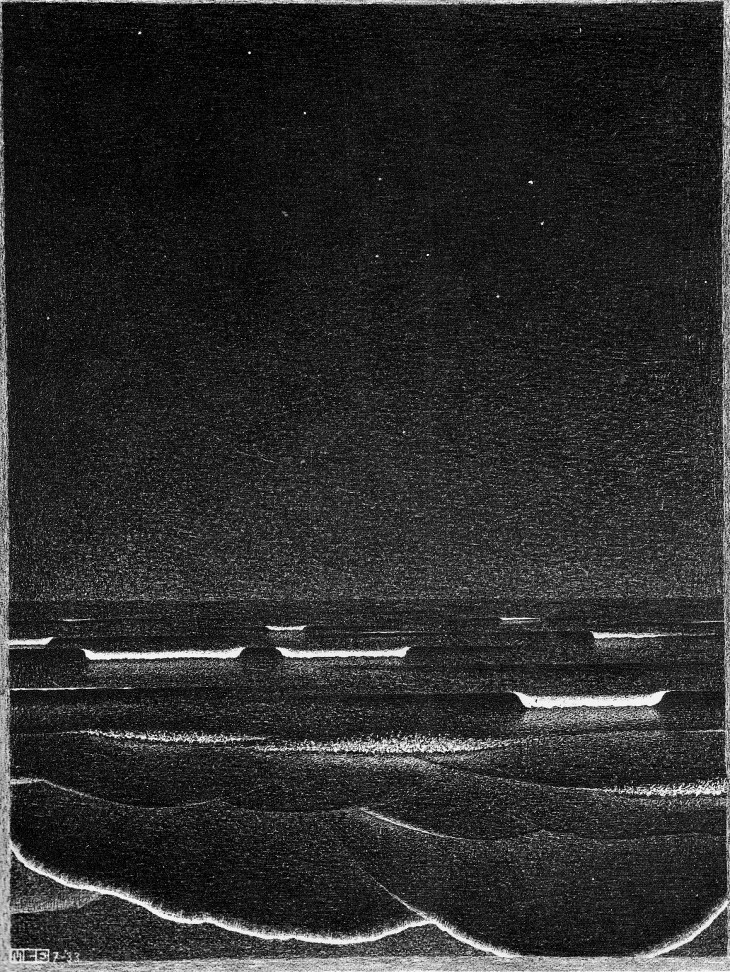
\includegraphics[scale=1.2]{escherOndas}

%----------------------------------------------------------------------------------------

\vfill % Fill the rest of the page with whitespace

\end{titlepage}

% ---------------------------------------------------------------------------------------
%         HEADER
%----------------------------------------------------------------------------------------

\fancyhead[L]{Favio Vázquez}
\fancyhead[R]{\thepage}

%----------------------------------------------------------------------------------------
\setcounter{footnote}{0}
\renewcommand*{\thefootnote}{\arabic{footnote}}
%----------------------------------------------------------------------------------------

%----------------------------------------------------------------------------------------
%%			BEGIN DOCUMENT
%----------------------------------------------------------------------------------------

\section{Problema 1. Problema 7.2 de Classical Electromagnetic Radiation
de Jackson \cite{jackson}.}

Una onda plana incidente en una interfaz de capas como se muestra en la figura. Los 
índices de refracción de los tres medios no impermeables son $n_1$, $n_2$ y $n_3$. 
El grosor de la capa intermedia es $d$. Cada uno de los otros medios es semi-infinito.

\begin{enumerate}[label=\textbf{(\alph*)}]
 \item Calcule los coeficientes de transmisión y reflexión (las tasas de del flujo de 
 Poynting transmitida y reflejada al flujo incidente), y esboce su comportamiento como 
 función de la frecuencia para $n_1 = 1$, $n_2 = 2$, $n_3 = 3$; $n_1 = 3$, $n_2 = 2$, 
 $n_3 = 1$ y $n_1 = 2$, $n_2 = 4$, $n_3 = 1$.

\begin{figure}[H]
 \center 
 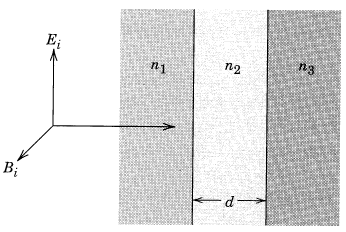
\includegraphics[scale=0.7]{problema1fig1}
\end{figure}

\item El medio $n_1$ es parte de un sistema óptico (e.g., una lente); el medio 
$n_3$ es aire $(n_3 = 1)$. Se desea colocar un revestimiento óptico (medio $n_2$) 
sobre la superficie para que no haya reflexión para ondas de frecuencia $\omega_0$. 
¿Qué grosor $d$ e índice de refracción $n_2$ son necesarios?

\end{enumerate}

\vspace{.3cm}

\underline{Solución:} \vspace{.3cm}

\textbf{(a)} Hago notar de que no encuentro una manera simple de hacer este problema, y el mecanismo 
que utilicé para solucionarlo fue inspirado en un texto que se llama ``A Companion 
to J.D. Jackson's Classical Electrodynamics'', de R. Magyar \cite{magyar}. En la 
discusión del capítulo 7 del texto de Jackson \cite{jackson}, argumenta algunas cosas interesantes que 
pueden utilizarse para resolver este problema, y aunque su discusión es mucho más 
extensa, la condensé para esta solución. Comencemos entonces.

\vspace{.3cm}

Como dice el enunciado, una onda electromagnética incide desde la izquierda y viaja 
por las capas; debido a que tratamos con una onda electromagnética sabemos que 
$\mathbf{k} \times \hat{\mathbf{n}} = 0$ y $\mathbf{B} \cdot \mathbf{E} = 0$, lo 
cual nos dice que $\mathbf{E}$ y $\mathbf{B}$ son perpendiculares al movimiento 
de la onda y son mutuamente perpendiculares entre ellas. Ya que los tres medios 
son no-permeables tenemos que $\mu_1 = \mu_2 = \mu_3 = 1$ y por lo tanto el 
índice de refracción para cara medio solo dependerá de las $\epsilon_i$. 

\vspace{.3cm}

Pensemos ahora en el recorrido de la onda por las capas. La primera capa puede reflejar 
la onda y contribuir directamente al coeficiente de reflexión efectivo, o también 
puede transmitir la onda. La segunda capa también puede reflejar la onda, si esto 
ocurre viajará de vuelta a la primera capa y puede ser transmitida a la misma. O 
la onda puede ser reflejada de vuelta. Y esto ocurre también si consideramos la 
tercera capa, por lo que vemos que el coeficiente de reflexión consistirá en una 
serie infinita de términos, donde cada término corresponde a una cierta cantidad 
de rebotes entre las capas antes de que la onda es finalmente reflejada a la 
izquierda. 

\vspace{.3cm}

Podemos escribir esto como 

\begin{equation}
r = r_{12} + t_{12}r_{23}t_{21} \euler^{2ik_2d} + t_{12}r_{23}r_{21}t_{21}
\euler^{4ik_2d} + \dots
\label{eq:reflex1}
\end{equation}

El primer término de esta ecuación corresponde a la reflexión en la interfaz 
$n_1-n_2$, el segundo término representa una onda que para por la interfaz 
$n_1-n_2$, se refleja en la interfaz $n_2-n_3$, y luego viaja de vuelta a la 
interfaz $n_1-n_2$, y así sucesivamente podemos imaginarnos los términos 
que corresponden a múltiples reflexiones internas. En esta ecuación vemos 
el cambio de fase, relacionado con $k_2 = n_2 \omega /c$, que en el primer 
término es el producto de los cambios ya que al llegar la onda va con $ikd$ y 
al devolverse va con $i(-k)(-d)$, por lo tanto el cambio total de fase será 
$2ikd$. Si escribimos la ecuación \eqref{eq:reflex1} como 

\begin{equation}
 r = r_{12} + [t_{12}r_{23}t_{21} \euler{2ik_2d}][1 + r_{23}r_{21}\euler{2ik_2d} 
 + (r_{23}r_{21})^2 \euler{4ik_2d} + \dots],
\end{equation}

y viendo que el segundo término es una serie geométrica que puede escribirse como 

\begin{equation}
 \sum_0^\infty x^n = \frac{1}{1-x},
\end{equation}

nos queda que, con $x = r_{23}r_{21}\euler^{2ik_2d}$,

\begin{equation}
 r = r_{12} + [t_{12}r_{23}t_{21} \euler^{2ik_2d}]\left[\frac{1}{1 - 
 r_{23}r_{21}\euler^{2ik_2d}} \right].
\end{equation}

De la ecuación (7.42) de Jackson \cite{jackson} vemos que 

\begin{equation}
 r_{ij} = \frac{n_i - n_j}{n_i + n_j},
\end{equation}

y 

\begin{equation}
 t_{ij} = \frac{2n_i}{n_i + n_j}.
\end{equation}

Con estas ecuaciones podemos mostrar que 

\begin{equation}
 r_{12} = \frac{n_1 - n_2}{n_1 + n_2} = - \frac{n_2 - n_1}{n_1 + n_2} = - r_{21},
\end{equation}

y que 

\begin{equation}
 t_{12}t_{21} = \left(\frac{2n_1}{n_1 + n_2} \right)\left(\frac{2n_1}{n_1 + n_2}\right) = 
 \frac{4 n_1 n_2}{(n_1 + n_2)^2} = 1 - \frac{(n_1 - n_2)^2}{(n_1 + n_2)^2} = 1 + r_{12}r_{21}.
\end{equation}

Por lo tanto podemos escribir 

\begin{equation}
 r = r_{12} + \frac{(1 + r_{12}r_{21})\euler^{2ik_2d}}{1 + r_{12}r_{23}\euler^{2ik_2d}} = 
 \frac{r_{12} + r_{23}\euler^{2ik_2d}}{1 + r_{12}r_{23}\euler^{2ik_2d}}.
\end{equation}

El coeficiente de reflexión se define como $R = |r|^2$, por lo tanto 

\begin{equation}
 \boxed{R = \frac{r_{12}^2 + r_{23}^2 + 2r_{12}r_{23}\cos{(2k_2d)}}{1 + 2r_{12}r_{23} 
 \cos{(2k_2d)} + (r_{12}r_{23})^2}},
\end{equation}

y debido a que $R + T = 1$ el coeficiente de transmisión resulta en 

\begin{equation}
 \boxed{T = \frac{1 - r_{12}^2 - r_{23}^2 + (r_{12}r_{23})^2}{1 + 2r_{12}r_{23}\cos{(2k_2d)} 
 + (r_{12}r_{21})^2}}.
\end{equation}

Necesitamos ahora hacer una serie de gráficos para el comportamiento de los coeficientes 
de reflexión y transmisión que encontramos para distintos índices de refracción. 

\vspace{.3cm}

Si $n_1 = 1$, $n_2 = 2$ y $n_3 = 3$, haciendo $d = 1c$ nos queda 

\begin{equation}
 R = \frac{1/4 + 1/25 + 1/5\cos{4\omega}}{1 + 1/100 + 1/5\cos{4\omega}},
\end{equation}

y 

\begin{equation}
 T = \frac{1 - 1/4 - 1/25 + (1/10)^2}{1 + 1/100 + 1/5\cos{4\omega}}
\end{equation}

cuyo gráfico es 

\begin{figure}[H]
 \center 
 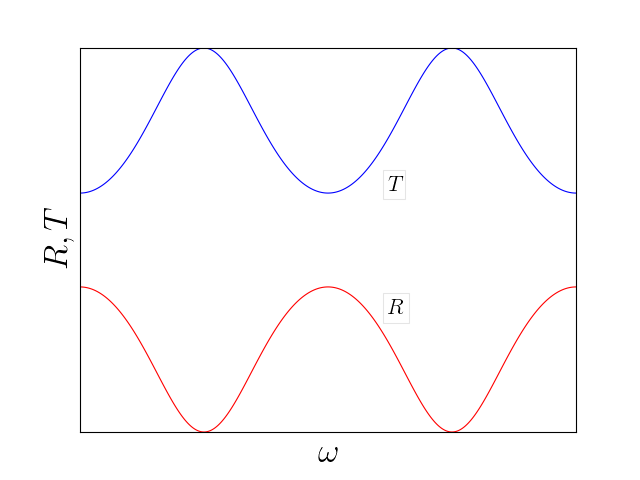
\includegraphics[scale=0.5]{problema1fig2}
 \caption{Coeficientes de reflexión y transmisión para $n_1 = 1$, $n_2 = 2$ y $n_3 = 3$.}
\end{figure}

Si $n_1 = 3$, $n_2 =2$ y $n_3 = 1$ nos queda

\begin{equation}
 R = \frac{1/4 + 1/25 + 1/5\cos{4\omega}}{1 + 1/100 + 1/5\cos{4\omega}},
\end{equation}

y 

\begin{equation}
 T = \frac{1 - 1/4 - 1/25 + (1/10)^2}{1 + 1/100 + 1/5\cos{4\omega}}
\end{equation}

cuyo gráfico es el mismo que en el anterior caso 

\begin{figure}[H]
 \center 
 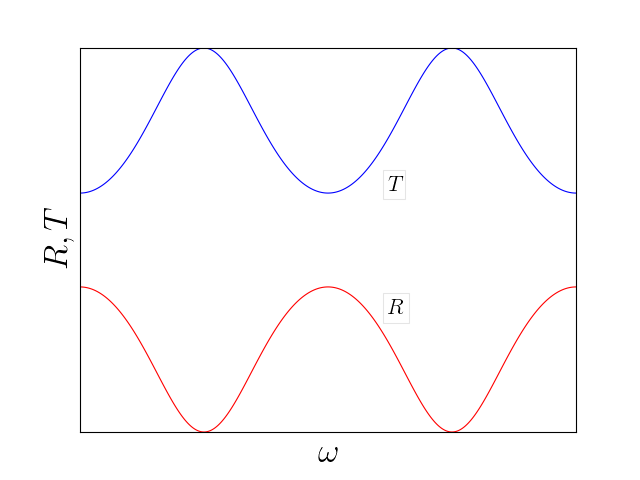
\includegraphics[scale=0.5]{problema1fig2}
 \caption{Coeficientes de reflexión y transmisión para $n_1 = 3$, $n_2 = 2$ y $n_3 = 1$.}
\end{figure}

Si $n_1 = 2$, $n_2 =4$ y $n_3 = 1$ nos queda

\begin{equation}
 R = \frac{1/9 + 9/25 - 2/5\cos{8\omega}}{1 + 1/25 - 2/5\cos{8\omega}},
\end{equation}

y 

\begin{equation}
 T = \frac{1 - 1/9 - 9/25 + 1/25}{1 + 1/25 - 2/5\cos{8\omega}}
\end{equation}

cuyo gráfico es 

\begin{figure}[H]
 \center 
 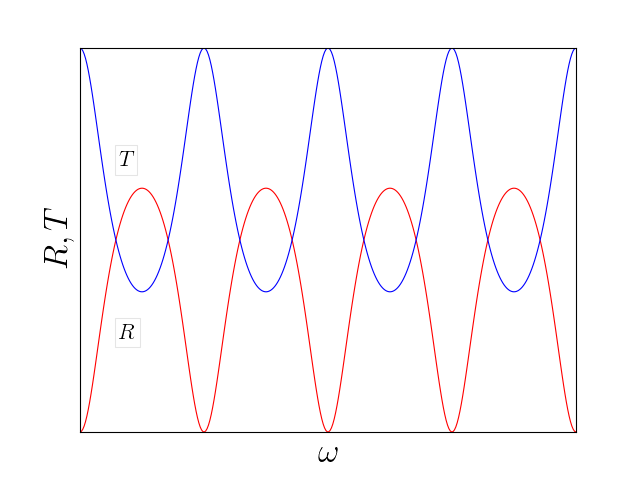
\includegraphics[scale=0.5]{problema1fig3}
 \caption{Coeficientes de reflexión y transmisión para $n_1 = 2$, $n_2 = 4$ y $n_3 = 1$.}
\end{figure}

El código para hacer estas imágenes se encuentra en un repositorio público el cual 
administro, donde también están los PDF de todas las tareas, así como el código 
\LaTeX \space con el que las hago. La página es: 
\href{https://github.com/FavioVazquez/Electrodinamica-Clasica-PCF}{https://github.com/FavioVazquez/Electrodinamica-Clasica-PCF}.
Los códigos están en NoteBooks de Python 3, los cuales GitHub renderiza de forma 
automática y pueden verse en línea.

\vspace{.3cm} 

El código que hace las primeras dos imágenes es:

\begin{lstlisting}[language=Python]
from __future__ import print_function
import numpy as np
from numpy import arccos,sin, cos, pi, array, sqrt
import matplotlib
matplotlib.use('nbagg')
import matplotlib.pyplot as plt
from matplotlib import rc

rc('font',**{'family':'sans-serif','sans-serif':['Helvetica']})
## for Palatino and other serif fonts use:
#rc('font',**{'family':'serif','serif':['Palatino']})
rc('text', usetex=True)

#LaTeX
plt.rc('text', usetex=True)
plt.rc('font', family='serif')

# Case n_1 = 1, n_2 = 2, n_3 = 3 and n_1 = 3, n_2 = 2, n_3 = 3.

# linespace for omega 
omega = np.linspace(0,pi,360)

# Def. of R and T
R_1 = (1/4 + 1/25 + 1/5*cos(4*omega))/(1 + 1/100 + 1/5*cos(4*omega))
T_1 = (1 - 1/4 - 1/25 + 1/100)/(1 + 1/100 + 1/5*cos(4*omega))

# Style
plt.ylabel(r'$R,T$', fontsize=30)
plt.xlabel(r'$\omega$',fontsize=30)
plt.xticks([])
plt.yticks([])

# Legend
plt.text(0.4, 0.33, r"$R$", bbox=dict(facecolor='white', alpha=0.1),
         fontsize=20)
plt.text(0.4, 0.65, r"$T$", bbox=dict(facecolor='white', alpha=0.1),
         fontsize=20)

# Plot
plt.plot(omega,R_1,"red",omega,T_1,"blue")
plt.show()
\end{lstlisting}

\newpage

El código que hace la segunda imagen es:

\begin{lstlisting}[language=Python]
from __future__ import print_function
import numpy as np
from numpy import arccos,sin, cos, pi, array, sqrt
import matplotlib
matplotlib.use('nbagg')
import matplotlib.pyplot as plt
from matplotlib import rc

rc('font',**{'family':'sans-serif','sans-serif':['Helvetica']})
## for Palatino and other serif fonts use:
#rc('font',**{'family':'serif','serif':['Palatino']})
rc('text', usetex=True)

#LaTeX
plt.rc('text', usetex=True)
plt.rc('font', family='serif')

# Case n_1 = 2, n_2 = 4, n_3 = 1

# linespace for omega 
omega = np.linspace(0,pi,360)

# Def. of R and T
R_2 = (1/9 + 9/25 - 2/5*cos(8*omega))/(1 + 1/25 - 2/5*cos(8*omega))
T_2 = (1 - 1/9 - 9/25 + 1/25)/(1 + 1/25 - 2/5*cos(8*omega))

# Style
plt.ylabel(r'$R,T$', fontsize=30)
plt.xlabel(r'$\omega$',fontsize=30)
plt.xticks([])
plt.yticks([])

# Legend
plt.text(0.25, 0.3, r"$R$", bbox=dict(facecolor='white', alpha=0.1),fontsize=20)
plt.text(0.25, 0.65, r"$T$", bbox=dict(facecolor='white', alpha=0.1),fontsize=20)

# Plot
plt.plot(omega,R_2,"red",omega,T_2,"blue")
plt.show()
\end{lstlisting}

\textbf{(b)} Si $n_3 = 1$ el coeficiente de reflexión se reduce a 

\begin{equation}
 R = 1 - \frac{8n_1 n_2^2}{n_1^2 + [1 + n_1(4 + n_1)]n_2^2 + n_2^4 + 
 (n_1 - n_2)(n_1 + n_2)(n_2^2 - 1)\cos{(2 d n_2 \omega_0)}}
\end{equation}

donde hemos cambiado $\omega$ por $\omega_0$ como lo especifica el inciso. Ahora 
si podemos hacer que $\cos{(2 d n_2 \omega_0)} = -1$ el requerimiento de que $R = 0$ 
se reduce a 

\begin{equation}
 n_1^2 + [1 + n_1(4 + n_1)]n_2^2 + n_2^4 + 
 (n_1 - n_2)(n_1 + n_2)(n_2^2 - 1) - 8n_1 n_2^2 = 0,
\end{equation}

lo que implica que $n_2 = \sqrt{n_1}$. Por lo tanto para que se cumpla que $R=0$, debemos 
escoger $n_2 = \sqrt{n_1}$ y para que se cumpla la condición que impusimos en el 
coseno, debe tenerse que $d = (m - 1/2)\frac{\pi}{\sqrt{n\omega_0}}$.

\newpage

\section{Problema 2. Problema 7.3 de Classical Electromagnetic Radiation
de Jackson \cite{jackson}.}

Dos losas planas semi-infinitas con el mismo dieléctrico sin pérdidas, uniformidad,
isotropía, no-permeabilidad con índice de refracción $n$ son paralelas, y están 
separadas por una brecha de aire ($n = 1$) de ancho $d$. Una onda electromagnética 
de frecuencia $\omega$ incide en la brecha desde una de las losas con un ángulo 
de incidencia $i$. Para una polarización lineal tanto paralela como perpendicular 
al plano de incidencia,

\begin{enumerate}[label=\textbf{(\alph*)}]
 \item calcule la tasa de potencia transmitida a la segunda losa con respecto 
 a la potencia incidente y la tasa de potencia reflejado con respecto a la incidente;
 \item para un $i$ mayor que el ángulo crítico para reflexión interna total, 
 esboce la tasa de potencia transmitida con respecto a la potencia incidente 
 como una función de $d$ medido en unidades de longitud de onda en la brecha.
\end{enumerate}

\vspace{.3cm}

\underline{Solución:} \vspace{.3cm}

\textbf{(a)} Asumiremos que la onda incidente puede escribirse como $\mathbf{E}_i 
\euler^{i\mathbf{k}\cdot \mathbf{x}}$, y del lado de la primera losa se refleja 
una onda de la forma  $\mathbf{E}_r \euler^{i\mathbf{k'}\cdot \mathbf{x}}$, luego 
en la brecha de aire tenemos las ondas  $\mathbf{E}_+
\euler^{i\mathbf{k}_0\cdot \mathbf{x}}$ y  $\mathbf{E}_- 
\euler^{i\mathbf{k}_0\cdot \mathbf{x}}$, y por último en la segunda losa tendremos 
una onda transmitida de la forma  $\mathbf{E}_t 
\euler^{i\mathbf{k}\cdot (\mathbf{x} - \mathbf{d})}$.

\vspace{.3cm}

Si $i$ es el ángulo de incidencia, entonces el ángulo $r$ medido desde la normal 
en la brecha de aire  está dado por la ley de Snell, $n \sen{i} = \sen{r}$, y
debido a que las losas  tienen el mismo índice de refracción, el ángulo de
transmisión también será $i$. Tenemos que, por lo anterior

\begin{equation}
 \cos{r} = \sqrt{q - \sen^2{r}} = \sqrt{1 - n^2\sen^2{i}},
\end{equation}

lo que nos dice que $\cos{r}$ es puramente imaginario cuando $i$ es más grande 
que el ángulo crítico. El problema nos pide que calculemos $E_t/E_i$ y $E_r/E_i$, 
y para hacer esto tomaremos dos casos posibles, y utilizando las condiciones 
de frontera para las componentes paralelas de $\mathbf{E}$ y $\mathbf{H}$ podremos hacer
esto\footnote{Ver página 304 de Jackson \cite{jackson}}. El primer caso es 
cuando $\mathbf{E}$ es perpendicular al plano de incidencia, entonces en la
primera interfaz tenemos 

\begin{align}
  \begin{split}
  E^{\parallel} &: E_i + E_r = E_+ + E_-, \\
  H^{\parallel} &: n(E_i - E_r)\cos{i} = (E_+ - E_-)\cos{r},
  \end{split}
\end{align}

y en la segunda interfaz 

\begin{align}
  \begin{split}
  E^{\parallel} &: E_+\euler^{i\phi} + E_-\euler^{-i\phi} = E_t, \\
  H^{\parallel} &: (E_+\euler^{i\phi} - E_-\euler^{-i\phi})\cos{r} =
  nE_t \cos{i},
  \end{split}
\end{align}

donde hemos definido la fase 

\begin{equation}
 \phi = \mathbf{k}_0 \cdot \mathbf{d} = k_0 d \cos{r} = \frac{\omega d \cos{r}}{c}.
\end{equation}

Ahora las ecuaciones para la primera interfaz podemos escribirlas como 

\begin{align}
 \begin{split}
  E_+ = \frac{1}{2}E_i(1 + \xi) + \frac{1}{2}E_r(1 - \alpha), \\
  E_- \frac{1}{2}E_i(1 - \xi) + \frac{1}{2}E_r(1 + \alpha),
 \end{split}
\end{align}

donde hemos definido 

\begin{equation}
 \xi \equiv \frac{n \cos{i}}{\cos{r}} = \frac{n\cos{i}}{\sqrt{1 - n^2\sen^2{i}}}.
\end{equation}

De igual forma las ecuaciones para la segunda interfaz podemos escribirlas como 

\begin{align}
 \begin{split}
  E_+ = \frac{1}{2}\euler^{-i\phi}E_t(1 + \xi), \\
  E_- = \frac{1}{2}\euler^{-i\phi}E_t(1 + \xi).
 \end{split}
\end{align}

Con estos dos pares de ecuaciones podemos resolver para las tasas solicitadas 
por el texto,

\begin{equation}
 \boxed{\frac{E_t}{E_i} = \frac{2\xi}{2\xi\cos{\phi} - i(1 + \xi^2)\sen{\phi}}},
\end{equation}

\begin{equation}
 \boxed{\frac{E_r}{E_i} = \frac{i(1 - \xi^2)\sen{\phi}}{2\xi\cos{\phi} - i(1 + \xi^2)
 \sen{\phi}}}.
\end{equation}

Como no me queda muy claro si el texto pide estas tasas solamente o también los 
coeficientes de reflexión y transmisión, debajo se encuentran éstos\footnote{Para 
los casos en que $i$ es menor que el ángulo crítico, y tanto $\xi$ como $\phi$ son 
reales.}

\begin{equation}
 \boxed{T = \left|\frac{E_t}{E_i} \right|^2 = \frac{4\xi^2}{4\xi^2 + 
 (1 - \xi)^2\sen^2{\phi}}},
\end{equation}

\begin{equation}
 \boxed{R = \left|\frac{E_r}{E_i} \right|^2 = \frac{(1 - \xi)^2\sen^2{\phi}}{4\xi^2 + 
 (1 - \xi)^2\sen^2{\phi}}}.
\end{equation}

Ahora para $\mathbf{E}$ paralelo al plano de incidencia, tenemos para la primera 
interfaz 

\begin{align}
 \begin{split}
  E^{\parallel} : (E_i - E_r)\cos{i} = (E_+ - E_-)\cos{r}, \\
  H^{\parallel} : n(E_i + E_r) = E_+ + E_-,
 \end{split}
\end{align}

y en la segunda interfaz 

\begin{align}
 \begin{split}
  (E_+ \euler^{i\phi} - E_-\euler^{-i\phi})\cos{r} = E_t \cos{i}, \\
  E_+ \euler^{i\phi} - E_-\euler^{-i\phi} = n E_t.
 \end{split}
\end{align}

De nuevo estas ecuaciones podemos escribirlas como 

\begin{align}
 \begin{split}
  n^{-1} E_+ = \frac{1}{2}E_i(1 + \zeta) + \frac{1}{2}E_r(1 - \zeta), \\
  n^{-1} E_- = \frac{1}{2}E_i(1 - \zeta) + \frac{1}{2}E_r(1 + \zeta), \\
 \end{split}
\end{align}

y 

\begin{align}
 \begin{split}
  n^{-1} E_+ = \frac{1}{2}\euler^{-i\phi}E_t(1 + \xi), \\
  n^{-1} E_- = \frac{1}{2}\euler^{-i\phi}E_t(1 + \xi).
 \end{split}
\end{align}

donde hemos definido 

\begin{equation}
 \zeta \equiv \frac{\cos{i}}{n\cos{r}} = \frac{\cos{i}}{n\sqrt{1 - n^2 \sen^{i}}}.
\end{equation}

Vemos que son ecuaciones muy similares a las que obtuvimos anteriormente solo con 
la diferencia de que en vez de $E_{\pm}$ tenemos $n^{-1}E_{\pm}$ y en vez de $\xi$ 
tenemos $\zeta$, y obtendremos las siguientes relaciones 

\begin{equation}
 \boxed{\frac{E_t}{E_i} = \frac{2\zeta}{2\zeta\cos{\phi} - i(1 + \zeta^2)\sen{\phi}}},
\end{equation}

\begin{equation}
 \boxed{\frac{E_r}{E_i} = \frac{i(1 - \zeta^2)\sen{\phi}}{2\zeta\cos{\phi} - i(1 + \zeta^2)
 \sen{\phi}}}.
\end{equation}

Y los coeficientes de reflexión y transmisión serán 

\begin{equation}
 \boxed{T = \left|\frac{E_t}{E_i} \right|^2 = \frac{4\zeta^2}{4\zeta^2 + 
 (1 - \zeta)^2\sen^2{\phi}}},
\end{equation}

\begin{equation}
 \boxed{R = \left|\frac{E_r}{E_i} \right|^2 = \frac{(1 - \zeta)^2\sen^2{\phi}}{4\zeta^2 + 
 (1 - \zeta)^2\sen^2{\phi}}}.
\end{equation}

\textbf{(b)} Como no se especifica, solo consideraremos el caso en que $\mathbf{E}$ es
perpendicular al plano de incidencia. Como $i$ es mayor que el ángulo crítico, tanto 
$\xi$ como $\phi$ son puramente imaginarios. Por simplicidad podemos escribir éstos 
como $\xi = i\gamma$, $\phi = i\beta$, entonces 

\begin{equation}
 \boxed{\frac{E_t}{E_i} = \frac{2i\gamma}{2i\gamma\cosh{\beta} - (1 - \gamma^2)\senh{\beta}}},
\end{equation}

\begin{equation}
 \boxed{\frac{E_r}{E_i} = \frac{-(1 + \gamma^2)\senh{\beta}}{2i\gamma\cosh{\beta} + (1 + \gamma^2)
 \sen{\beta}}}.
\end{equation}

Y los coeficientes de reflexión y transmisión quedan como

\begin{equation}
 \boxed{T = \left|\frac{E_t}{E_i} \right|^2 = \frac{4\gamma^2}{4\gamma^2 + 
 (1 - \gamma)^2\senh^2{\beta}}},
\end{equation}

\begin{equation}
 \boxed{R = \left|\frac{E_r}{E_i} \right|^2 = \frac{(1 - \gamma)^2\senh^2{\beta}}{4\gamma^2 + 
 (1 - \gamma)^2\senh^2{\beta}}}.
\end{equation}

Donde, 

\begin{equation}
 \gamma = - \frac{n\cos{i}}{\sqrt{n^2\sen^2{i} -1}},
\end{equation}

y

\begin{equation}
 \beta = \frac{\omega d \sqrt{n^2 \sen^2{i} -1}}{c}.
\end{equation}

Para tomar un ejemplo, podemos usar que en el aire, con índice de refracción 
$n \approx 1.5$ el ángulo crítico para la reflexión total interna es de $i_0 = 42^\circ$. 
Y el gráfico de $T$ en función de $d$ medido en unidades de longitud de onda en la 
brecha será 

\begin{figure}[H]
 \center 
 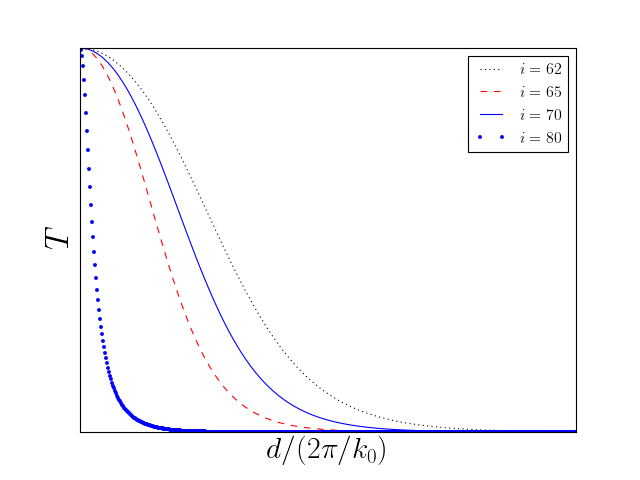
\includegraphics[scale=0.5]{problema2fig1}
 \caption{Coeficiente de transmisión para $n \approx 1.5$ en función de $d$.}
\end{figure}

El código que esta imagen es:

\begin{lstlisting}[language=Python]
from __future__ import print_function
import numpy as np
from numpy import arccos,sin, cos, pi, array, sqrt
import matplotlib
matplotlib.use('nbagg')
import matplotlib.pyplot as plt
from matplotlib import rc

rc('font',**{'family':'sans-serif','sans-serif':['Helvetica']})
## for Palatino and other serif fonts use:
#rc('font',**{'family':'serif','serif':['Palatino']})
rc('text', usetex=True)

#LaTeX
plt.rc('text', usetex=True)
plt.rc('font', family='serif')

# Linespace for d
d = np.linspace(0,10,500)

# Variable definitions

def gamma(angle):
    return - (1.5 * cos(angle)) / sqrt((1.5**2)*(sin(angle))**2-1)

def beta(angle):
    return d*sqrt((1.5**2)*(sin(angle)**2) - 1)

T1 = (5*gamma(62)**2) / ((4 * gamma(62)**2) + (1+gamma(62)**2) * 
                         sinh(beta(62))**2)

T2 = (5*gamma(65)**2) / ((4 * gamma(65)**2) + (1+gamma(65)**2) * 
                         sinh(beta(65))**2)

T3 = (5*gamma(70)**2) / ((4 * gamma(70)**2) + (1+gamma(70)**2) * 
                         sinh(beta(70))**2)

T4 = (5*gamma(80)**2) / ((4 * gamma(80)**2) + (1+gamma(80)**2) * 
                         sinh(beta(80))**2)

# Style
plt.ylabel(r'$T$', fontsize=30)
plt.xlabel(r'$d$',fontsize=30)
plt.xticks([])
plt.yticks([])

# Legend
plt.legend(handles=[T1plot,T2plot,T3plot,T4plot], loc=1)

# Plot
T1plot, = plt.plot(d,T1,"k:", label = "$i = 62$")
T2plot, = plt.plot(d,T2,"r--", label = "$i = 65$")
T3plot, = plt.plot(d,T3,"b", label = "$i = 70$")
T4plot, = plt.plot(d,T4,".", label = "$i = 80$")
plt.show()
\end{lstlisting}

\newpage

\section{Problema 3. Problema 7.5 de Classical Electromagnetic Radiation
de Jackson \cite{jackson}.}

Una onda electromagnética polarizada $\mathbf{E} = \mathbf{E}_i \euler^{i\mathbf{k}} 
\cdot \mathbf{x} - i\omega t$ incide normalmente sobre una lámina plana uniforme 
de una excelente conducción ($\omega \gg \omega \epsilon_0$) con un grosor de $D$. 
Asumiendo que en el espacio y en la lámina conductora $\mu/\mu_0 = \epsilon/\epsilon_0 
= 1$, discuta la reflexión y transmisión de la onda incidente. 

\begin{enumerate}[label=\textbf{(\alph*)}]
 \item Muestre que las amplitudes de las onda reflejada y transmitida, correctas 
 a primer orden en $(\epsilon_0 \omega /\sigma)^{1/2}$, son 
 
 $$
 \frac{E_r}{E_i} = \frac{-(1 - \euler^{-2\lambda})}{(1 - \euler^{-2\lambda}) 
 + \gamma(1 + \euler^{-2\lambda})}
 $$
 
  $$
 \frac{E_t}{E_i} = \frac{2\gamma \euler^{-\lambda}}{(1 - \euler^{-2\lambda}) 
 + \gamma(1 + \euler^{-2\lambda})}
 $$
 
 donde 
 
 $$
 \gamma = \sqrt{\frac{2\epsilon_0 \omega}{\sigma}}(1 - i) = \frac{\omega \delta}{c}
 (1 - i)
 $$
 
 $$
 \lambda = (1-i)D/\delta
 $$
 
  y $\delta = \sqrt{2/\omega \mu \sigma}$ es la profundidad de penetración.
 
 \item Verifique que para un grosor igual a cero y un grosor infinito se obtienen 
 los resultados limitantes apropiados.
 \item Muestre que, excepto para láminas de muy poco grosor, el coeficiente de 
 transmisión es 
 
 $$
 T = \frac{8(\text{Re} \gamma)^2 \euler^{-2D/\delta}}{1 - 2\euler^{-2D/\delta} 
 (\cos{2D/\delta) + \euler^{-4D/\delta}}}
 $$
\end{enumerate}

Esboce log $T$ como una función de $(D/\delta)$, asumiendo que Re $\gamma = 10^{-2}$. 
Defina ``grosor muy pequeño''.

\vspace{.3cm}

\underline{Solución:} \vspace{.3cm}

\textbf{(a)} Mientras consideremos que la lámina conductora como un medio con 
constante dieléctrica compleja 

\begin{equation}
 \epsilon/\epsilon_0 = 1 + i\frac{\sigma}{\omega \epsilon_0},
\end{equation}

podemos trabajar como si todo fuera un dieléctrico. Vemos entonces que este problema 
es muy similar al anterior y procedemos de la misma manera. Introduciremos los 
campos vectoriales de la forma $\mathbf{E}_i \euler^{i\mathbf{k} \cdot \mathbf{x}}$ 
y $\mathbf{E}_r \euler^{- i\mathbf{k} \cdot \mathbf{x}}$ en la zona de incidencia, 
$\mathbf{E}_+ \euler^{i\mathbf{k}_1 \cdot \mathbf{x}}$ y 
$\mathbf{E}_- \euler^{-i\mathbf{k}_1 \cdot \mathbf{x}}$ en la lámina conductora y 
$\mathbf{E}_t \euler^{i\mathbf{k} \cdot (\mathbf{x} - \mathbf{D})}$ en el lado 
de transmisión. Utilizamos ahora las condiciones de acople para la parte perpendicular 
de $\mathbf{E}$ al plano de incidencia. Tenemos entonces, para la primera interfaz 

\begin{align}
 E^\parallel &: E_i + E_r = E_+ + E_-, \\
 H^\parallel &: (E_i - E_r) = n(E_+ - E_-).
\end{align}

Y para la segunda interfaz, 

\begin{align}
 E_+ \euler^{i\phi} + E_- \euler^{-i\phi} &= E_t, \\
 n (E_+ \euler^{i\phi} - E_- \euler^{-i\phi}) &= E_t,
\end{align}

donde $n$ es el índice de refracción complejo 

\begin{equation}
 n = \sqrt{\frac{\epsilon}{\epsilon_0}} = \sqrt{1 + i \frac{\sigma}{\omega\epsilon_0}},
\end{equation}

y $\phi$ es la fase  de cambio al atravesar el dieléctrico 

\begin{equation}
 \phi = k_1 D = \frac{\omega n}{c} D = \frac{\omega D}{c}\sqrt{1 + i 
 \frac{\sigma}{\omega\epsilon_0}}.
\end{equation}

Resolviendo ahora para $E_t$ y $E_r$ en términos de $E_i$ obtenemos 

\begin{equation}
 \frac{E_t}{E_i} = \frac{4/n \euler^{i\phi}}{(1 + 1/n^2)(1 - \euler^{2i\phi}) 
 + 2/n (1 + \euler^{2i\phi})},
\end{equation}

\begin{equation}
  \frac{E_r}{E_i} = \frac{-(1 - 1/n^2)(1- \euler^{2i\phi})}{(1 + 1/n^2)(1 - \euler^{2i\phi}) 
 + 2/n (1 + \euler^{2i\phi})}.
\end{equation}

Tomando ahora el límite utilizando lo que dice el enunciado de que la lámina es 
un conductor excelente, $\sigma/\omega \epsilon_0 \gg 1$. En este caso el índice 
de refracción y la fase de cambio se aproximan por 

\begin{equation}
 n \approx (1 + i) \sqrt{\frac{\sigma}{2\epsilon_0 \omega}} = \frac{2}{\gamma},
\end{equation}

\begin{equation}
 \phi \approx (1 + i) D \sqrt{\frac{\mu_0 \sigma \omega}{2}} = i \lambda,
\end{equation}

donde hemos utilizado la definición de $\gamma$ y $\lambda$ que da el enunciado del 
problema. Para $|\gamma| \ll 1$ y despreciando términos del orden $\mathcal{O}(1/n^2)$ 
comparado a $1$ y sustituyendo arriba obtenemos 

\begin{equation}
 \boxed{\frac{E_r}{E_i} = \frac{-(1 - \euler^{-2\lambda})}{(1 - \euler^{-2\lambda}) 
 + \gamma(1 + \euler^{-2\lambda})}},
\end{equation}

\begin{equation}
  \boxed{\frac{E_t}{E_i} = \frac{2\gamma \euler^{-\lambda}}{(1 - \euler^{-2\lambda}) 
 + \gamma(1 + \euler^{-2\lambda})}}.
\end{equation}

\hspace{10cm}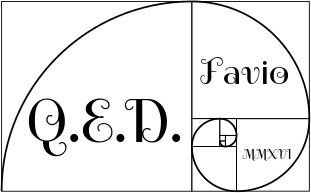
\includegraphics[scale=0.25]{logoQED}

\textbf{(b)} El grosor igual a cero corresponde a $\lambda \rightarrow 0$. En este 
caso, viendo las ecuaciones para $E_t/E_i$ y $E_r/E_i$ que obtuvimos en 
el inciso anterior, tenemos que 

\begin{equation}
 \frac{E_t}{E_i} \rightarrow 1,
\end{equation}

\begin{equation}
 \frac{E_r}{E_i} \rightarrow 0.
\end{equation}

Y en el caso de grosor infinito, es decir, $\lambda \rightarrow \infty$, tenemos que 

\begin{equation}
 \frac{E_t}{E_i} \rightarrow 0,
\end{equation}

\begin{equation}
 \frac{E_r}{E_i} \rightarrow - \frac{1}{1 + \gamma}.
\end{equation}

\hspace{10cm}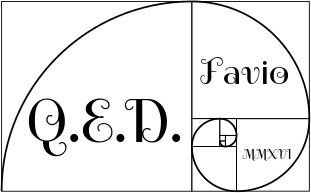
\includegraphics[scale=0.25]{logoQED}

La reflexión no se va a 1 en este casi ya que la lámina no es un un conductor perfecto 
y existe disipación de potencia (aunque muy poca). 

\vspace{.3cm}

\textbf{(c)} Para calcular el coeficiente de transmisión desde la expresión que 
obtuvimos para $E_t/E_i$ que obtuvimos en el inciso (b), debido a que $\gamma$ y 
$\lambda$ son complejos, y mientras no estemos en el límite para grosor muy 
pequeño, que definiremos pronto, los términos $\mathbf{O}(\gamma)$ pueden ser 
ignorados en el denominador. Entonces 

\begin{equation}
 \frac{E_t}{E_i} \approx \frac{2 \gamma \euler^{-\lambda}}{(1 - \euler^{-2\lambda})},
\end{equation}

de manera que 

\begin{equation}
 T = \left|\frac{E_t}{E_i} \right|^2 = \frac{4|\gamma|^2 \euler^{-2\text{Re}\lambda}}{
 1 - 2 \text{Re}(\euler^{-2\lambda} + \euler^{-4\text{Re} \lambda}},
\end{equation}

tomando ahora $|\gamma|^2 = 2(\text{Re} \gamma)^2$ y $\euler^{-2\lambda} 
= \euler^{2i D / \delta}\euler^{-2D/\delta}$ tenemos entonces 

\begin{equation}
 \boxed{T = \frac{8(\text{Re} \gamma)^2 \euler^{-2D/\delta}}{1 - 2\euler^{-2D/\delta} 
 (\cos{2D/\delta) + \euler^{-4D/\delta}}}}.
\end{equation}

\hspace{10cm}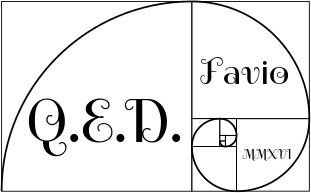
\includegraphics[scale=0.25]{logoQED}

El límite para grosor muy pequeño ocurre cuando los términos $\mathcal{O}(\gamma)$ 
se hacen importantes. Esto ocurre cuando 

\begin{equation}
 |1 - \euler^{-2\lambda}| \approx |\gamma(1 + \euler^{-2\lambda}|.
\end{equation}

Expandiendo para $\lambda$ pequeño 

\begin{equation}
 |2 \lambda| \approx |2 \gamma| \Rightarrow \frac{D}{\delta} \approx
 \frac{\omega \delta}{c}.
\end{equation}

Por lo tanto de lo anterior vemos que el límite para grosor muy pequeño, en este 
caso puede definirse como 

\begin{equation}
 \boxed{D < \frac{\omega \delta^2}{c}}.
\end{equation}

Debajo se encuentra el gráfico de log $T$ como una función de $(D/\delta)$, 
asumiendo que Re $\gamma = 10^{-2}$. 

\begin{figure}[H]
 \center 
 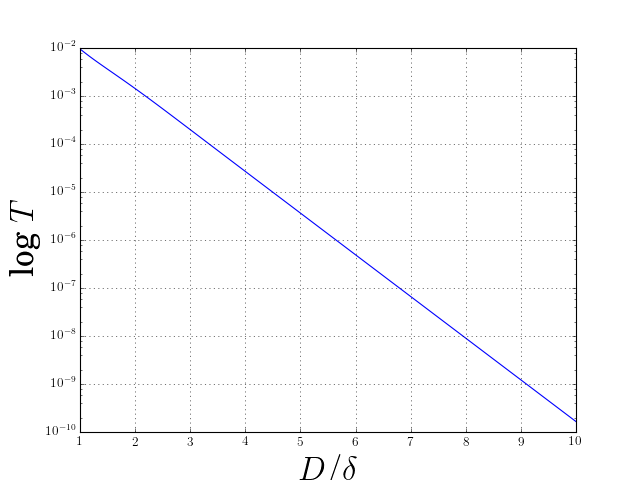
\includegraphics[scale=0.5]{problema3fig1}
 \caption{Gráfico de log $T$ como una función de $(D/\delta)$, 
asumiendo que Re $\gamma = 10^{-2}$.}
\end{figure}

Debajo se encuentra el código que hace la figura:

\begin{lstlisting}[language=Python]
from __future__ import print_function
import numpy as np
from numpy import arccos,sin, cos, pi, array, sqrt
import matplotlib
matplotlib.use('nbagg')
import matplotlib.pyplot as plt
from matplotlib import rc

rc('font',**{'family':'sans-serif','sans-serif':['Helvetica']})
## for Palatino and other serif fonts use:
#rc('font',**{'family':'serif','serif':['Palatino']})
rc('text', usetex=True)

#LaTeX
plt.rc('text', usetex=True)
plt.rc('font', family='serif')

# Linespace for Ddelta
Ddelta = np.linspace(1,10,500)

# Variable definitions

T = (8 * (10E-2)**2 * exp(-2*Ddelta)) / (1 - 
    (2 * exp(-2*Ddelta) * cos(2*Ddelta)) + exp(-4*Ddelta))

# Style
plt.ylabel(r'log $ T$', fontsize=30)
plt.xlabel(r'$D/\delta$',fontsize=30)

# Plot
T1plot, = plt.semilogy(Ddelta,T,"b")
plt.grid(True)
plt.show()

\end{lstlisting}

\newpage

\section{Problema 4. Problema 7.14 de Classical Electromagnetic Radiation
de Jackson \cite{jackson}. (Es el 7.9 de la 2da ed.)}

Un modelo simple para la propagación de ondas de radio en la atmósfera de la 
Tierra o ionosfera consiste en una tierra plana en $z = 0$ y un medio no 
uniforme con $\epsilon = \epsilon(z)$ para $z > 0$. Considere la ecuaciones 
de Maxwell bajo la suposición de que los campos son independientes de $y$ y 
pueden escribirse como funciones de $z$ por $\euler^{i(kx - \omega t)}$. 

\begin{enumerate}[label=\textbf{(\alph*)}]
 \item Muestre que la ecuación de onda que gobierna la propagación para $z > 0$ 
 es 
 
 $$
 \frac{d^2 F}{dz^2} + q^2(z) F = 0,
 $$
 
 donde 
 
 $$
 q^2(z) = \frac{\omega^2}{c^2}  - k^2
 $$
 
 y $F = E_y$ para la polarización \emph{horizontal}, y 
 
 $$
 q^2(z) =\frac{\omega^2}{c^2} \epsilon(z) + \frac{1}{2\epsilon}\frac{d^2 \epsilon}{dz^2} 
 - \frac{3}{4\epsilon^2}\left(\frac{d \epsilon}{d z} \right)^2 - k^2
 $$
 
 con $F = \sqrt{\epsilon}E_z$ para la polarización \emph{vertical}.
 
 \item Use la aproximación WKB para tratar la propagación de ondas dirigidas 
 verticalmente hacia la ionosfera ($k = 0$), asumiendo que la constante dieléctrica 
 está dada por (7.59) con una frecuencia de plasma $\omega_p(z)$ gobernada por una 
 densidad electrónica como se muestra en la figura 7.11. Verifique que los argumentos 
 cualitativos de la sección 7.6 se mantienen, con discrepancias en detalle solo 
 para $\omega ~ \omega_{p,\text{max}}$.
 
 \item Usando los resultados WKB de la parte (b) y los conceptos de propagación 
 de un pulso de la sección 7.8, define una altura efectiva de la ionosfera $h'(\omega)$ 
 calculando el tiempo $T$ para un pulso de frecuencia dominante $\omega$ que viaja 
 hacia arriba y se refleja ($h' \equiv cT/2)$. [La aproximación WKB es discutida 
 en la mayoría de los libros de mecánica cuántica].
\end{enumerate}

\vspace{.3cm}

\underline{Solución:} \vspace{.3cm}

\textbf{(a}) Comenzamos escribiendo las ecuaciones de Maxwell sin fuentes ($\rho = 
\mathbf{J} = 0$, con $\mu = 1$, 

\begin{align}
 \begin{split}
  \pmb{\nabla} \cdot (\epsilon \mathbf{E}) &= 0, \\
  \pmb{\nabla} \cdot \mathbf{B} &= 0, \\
  \pmb{\nabla} \times \mathbf{E} &= - \frac{1}{c} \frac{\partial \mathbf{B}}
  {\partial t}, \\
  \pmb{\nabla} \times \mathbf{B} &= - \frac{\epsilon}{c} \frac{\partial \mathbf{E}}
  {\partial t}.
 \end{split}
\end{align}

Para un medio no homogéneo tenemos 

\begin{equation}
 \pmb{\nabla} \epsilon \cdot \mathbf{E} + \epsilon \pmb{\nabla} \cdot \mathbf{E} = 
 0,
\end{equation}

que podemos escribir como 

\begin{equation}
 \frac{d \epsilon}{d z} E_z + \epsilon \pmb{\nabla} \cdot \mathbf{E} = 0.
\end{equation}

Ahora por propiedades del rotacional 

\begin{equation}
 \pmb{\nabla} \times ( \pmb{\nabla} \times \mathbf{E}) = 
 \pmb{\nabla} (\pmb{\nabla} \cdot \mathbf{E}) - \nabla^2 \mathbf{E} = 
 - \frac{1}{c} \frac{\partial}{\partial t} \left(\frac{\epsilon}{c} 
 \frac{\partial \mathbf{E}}{\partial t}\right),
\end{equation}

y entonces resultando lo obtenido arriba

\begin{equation}
 \nabla^2 \mathbf{E} - \frac{\epsilon}{c^2} \frac{\partial^2}{\partial t^2} \mathbf{E} = 
 \nabla \left(- \frac{1}{\epsilon} \frac{d\epsilon}{dz} E_z \right) = 
 - \frac{d}{dz} \ln{\epsilon} \nabla E_z - \hat{z} E_z \frac{d^2}{dz^2} \ln{\epsilon} ,
\end{equation}

\begin{equation}
 \therefore \mathbf{E} = \mathbf{E}(z) \euler^{i(kx - \omega t)}.
\end{equation}

Hemos probado entonces que lo que dice el enunciado para este tipo de ondas es cierto. 
Ahora, 

\begin{equation}
 \frac{d^2}{dz} \mathbf{E} + \left(\frac{\epsilon \omega}{c^2} - k^2 \right)\mathbf{E} = 
 - \frac{d}{dz} \ln{\epsilon} \frac{d}{dz} E_z \hat{z} - E_z \frac{d^2}{dz^2}
 \ln{\epsilon} \hat{z} = - \frac{d}{dz}\left(E_z \frac{d}{dz} \ln{\epsilon} \right) 
 \hat{z}.
\end{equation}

Para polarización horizontal tenemos que $E_y \ne 0$, entonces 

\begin{equation}
 \left[ \frac{d^2}{dz}  + \left(\frac{\epsilon \omega}{c^2} - k^2 \right)\right] E_y 
 = 0,
\end{equation}

o 

\begin{equation}
 \boxed{\left(\frac{d^2}{dz} + q^2(z) \right) E_y = 0},
\end{equation}

con 

\begin{equation}
 \boxed{q^2(z) = \frac{\epsilon \omega}{c^2} - k^2}.
\end{equation}

\hspace{10cm}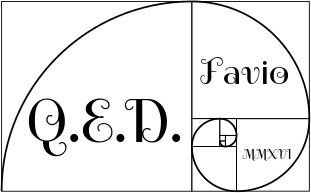
\includegraphics[scale=0.25]{logoQED}

Y para la polarización vertical tenemos que $E_z \ne 0$, entonces 

\begin{equation}
  \left[ \frac{d^2}{dz}  + \left(\frac{\epsilon \omega}{c^2} - k^2 \right)\right] E_z 
 = - \frac{d}{dz}\left(E_z \frac{d}{dz} \ln{\epsilon} \right),
\end{equation}

Si hacemos $E_z = F/\sqrt{\epsilon}$ obtenemos 

\begin{equation}
 \frac{d}{dz} E_z = \frac{1}{\sqrt{\epsilon}} \frac{d F}{dz} 
 - \frac{1}{2 \epsilon^{3/2}} F \frac{d\epsilon}{dz},
\end{equation}

y derivando de nuevo 

\begin{equation}
 \frac{d^2}{dz^2} E_z = \frac{1}{\sqrt{\epsilon}} \frac{d^2 F}{dz^2} - 
 \frac{1}{\epsilon^{3/2}}\frac{dF}{dz}\frac{d\epsilon}{dz} + 
 \frac{3}{4} \frac{F}{\euler^{3/2}} \left(\frac{d\epsilon}{dz} \right)^2 
 - \frac{F}{2\epsilon^{3/2}} \frac{d^2 \epsilon}{dz^2}.
\end{equation}

Con un poco de trabajo algebraico llegamos a 

\begin{equation}
 \frac{d^2}{dz^2} F + F \left\{\left(\frac{d\epsilon}{dz} \right)^2 
 \left(- \frac{3}{4\epsilon^2}\right) + \frac{d^2 \epsilon}{dz^2} 
 \frac{1}{2\epsilon} + \left[\frac{\epsilon\omega^2}{c^2} - k^2\right]\right\} = 0,
\end{equation}

o 

\begin{equation}
 \boxed{\frac{d^2 F}{dz^2} + q^2(z) F = 0},
\end{equation}

con

\begin{equation}
  \boxed{q^2(z) =\frac{\omega^2}{c^2} \epsilon(z) + \frac{1}{2\epsilon}\frac{d^2 \epsilon}{dz^2} 
 - \frac{3}{4\epsilon^2}\left(\frac{d \epsilon}{d z} \right)^2 - k^2}.
\end{equation}

\hspace{10cm}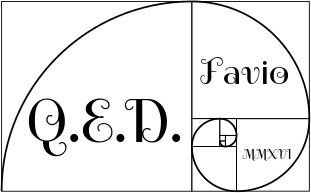
\includegraphics[scale=0.25]{logoQED}

\textbf{(b)} En Física, la aproximación WKB (Wentzel–Kramers–Brillouin)es el 
ejemplo más familiar de un cálculo semi-clásico en el cual la función de onda es 
redactada como una función exponencial, y entonces o la amplitud o la fase es
tomada para estar cambiando lentamente. Entonces tomando que 

\begin{equation}
 F = A \euler^{i\phi},
\end{equation}

\begin{equation}
 F' = i \phi' F,
\end{equation}

\begin{equation}
 F'' = i \phi'' F - \phi' F,
\end{equation}

y con la ecuación del anterior inciso, 

\begin{equation}
 F'' + q^2 F = 0 \Rightarrow (i\phi'' + \phi'^2 + q^2) F = 0,
\end{equation}

y en la aproximación WKB $\phi'' \approx 0$, por lo que 

\begin{equation}
 \phi' = q \Rightarrow \phi = \int dz q.
\end{equation}

Para una propagación vertical $k=0$, nos queda, utilizando los resultados del 
inciso anterior

\begin{equation}
 F = \sqrt{e} E_z \approx A \exp{\left[dz \sqrt{\frac{\epsilon \omega^2}{c^2}} 
 + \frac{1}{2\epsilon} \frac{d^2}{dz^2} - \frac{3}{4\epsilon^2} 
 \left(\frac{d\epsilon}{dz}\right)^2 \right]},
\end{equation}

\begin{equation}
 \therefore E_y \approx B \exp{[\int dz \frac{\omega}{c}\sqrt{\epsilon}]},
\end{equation}

Vemos entonces que 

\begin{equation}
 \epsilon \approx 1 - \frac{\omega_p^2}{\omega^2},
\end{equation}

donde, como en la ecuación (7.60) de Jackson \cite{jackson}

\begin{equation}
\omega_p^2 = 4\pi N Z \euler^2 /m,
\end{equation}

donde $NZ$ es el número total de electrones por unidad de volumen, y $e$ y $m$ 
son la carga y la masa del electrón, respectivamente. Vemos que a una frecuencia 
$\omega$ dada encontramos que $\epsilon > 0$ para $y$ pequeño y $\epsilon < 0$ 
para $y$ grande, siguiendo los argumentos de la sección 7.6 de Jackson \cite{jackson}. 

\vspace{.3cm}

\textbf{(c)} En este caso definimos el pulso por 

\begin{equation}
 E_+ = \int d\omega A(\omega) \frac{1}{\sqrt{q(\omega)}} \euler^{i\theta}, 
\end{equation}

donde la fase está dada por 

\begin{equation}
 \theta = \int dz q - \omega t,
\end{equation}

y la velocidad de fase a una frecuencia $\omega$ por 

\begin{equation}
 \frac{d\theta}{d\omega} = 0 = \frac{d}{d\omega} \int dz q - t = 
 \int dz \frac{dq}{d\omega} - t = \int dz \frac{1}{v_g} - t,
\end{equation}

donde hemos generalizado hacia la velocidad de grupo $v_g$, que se escribe como 

\begin{equation}
 \therefore v_g = \left(\frac{dq}{d\omega}\right)^{-1}.
\end{equation}

Por lo tanto el tiempo necesario para llegar a $z$ será 

\begin{equation}
 r = \int dz \frac{dq}{d\omega},
\end{equation}

pero 

\begin{equation}
 q = \frac{\omega}{c}\sqrt{\epsilon},
\end{equation}

y

\begin{equation}
 \frac{dq}{d\omega} = \frac{1}{v_g} = \frac{\sqrt{\epsilon}}{c} + \frac{\omega}{c} 
 \frac{1}{2\sqrt{\epsilon}} \frac{d\epsilon}{d\omega},
\end{equation}

y entonces el tiempo medio $T/2$ para un pulso de frecuencia dominante $\omega$ que
viaja hacia arriba y se refleja será 

\begin{equation}
 \frac{T}{2} = \int_0^{z'} dz \frac{1}{v_g},
\end{equation}

con la ecuación para la altura efectiva que da el texto encontramos que 

\begin{equation}
 h = \int_0^{z'} dz \left[\sqrt{\epsilon} + \frac{\omega}{2\sqrt{\epsilon}} 
 \frac{d\epsilon}{d\omega}\right].
\end{equation}

Ahora usando el resultado para $\epsilon$ del inciso anterior 

\begin{equation}
 \epsilon \approx = 1 - \frac{\omega_p^2}{\omega} = 1 - \xi^2,
\end{equation}

donde hemos definido $\xi \equiv \frac{\omega_p^2}{\omega}$. Por lo tanto 

\begin{equation}
 h = \int_0^{z'} dz \left[\sqrt{1 - \xi^2} + \xi^2 \frac{1}{\sqrt{1 - \xi^2}} \right],
\end{equation}

que podemos escribir como

\begin{equation}
 h = \int_0^{z'} dz \frac{1}{\sqrt{1 - \xi^2}},
\end{equation}

\begin{equation}
 \boxed{\therefore h = \int_0^{z'} dz \frac{\omega^2}{\sqrt{\omega^2 - \omega_p^2}}}.
\end{equation}

\newpage

\begin{thebibliography}{10}
\bibitem{jackson}
J. Jackson, \emph{Classical Electrodynamics}, 3ra edición. John Wiley and Sons, Inc. 
1999.
\bibitem{magyar}
R. Magyar, \emph{A Companion to Classical Electrodynamics 3rd Edition by J.D. 
Jackson}, 2001.
\end{thebibliography}

\end{document}